\documentclass[dvipdfmx,autodetect-engine]{article}
%---------------------package
\usepackage{geometry}
\usepackage{amssymb}
\usepackage{amsmath}
\usepackage{amsthm}
\usepackage{tikz}
\usetikzlibrary{positioning}

% ----------------------------- 
\theoremstyle{definition}
\newtheorem{Def}{定義}
\newtheorem{Th}{定理}
\newtheorem{Prop}{命題}
\newtheorem{Ex}{例}
\newtheorem{Cor}{系}
\newtheorem{Lem}{補題}
\newtheorem{Prob}{問}

% ------------------------- enumareteで(1)みたいにする
\renewcommand\labelenumi{(\arabic{enumi})}
\renewcommand\labelenumii{(\alph{enumii})}
\renewcommand\labelenumiii{(\roman{enumiii})}

%----------------------------命令定義
\DeclareMathOperator{\Hom}{Hom}
\DeclareMathOperator{\End}{End}
\DeclareMathOperator{\GL}{GL}
\DeclareMathOperator{\gl}{gl}
\DeclareMathOperator{\sllie}{sl}
\DeclareMathOperator{\sublie}{\mathfrak{a}}
\DeclareMathOperator{\lie}{\mathfrak{g}}
\DeclareMathOperator{\cartan}{\mathfrak{h}}
\DeclareMathOperator{\U}{U}


%---------------------------make title
\title{量子群の表現論}
\author{}
\date{}
%-----------------------------document
\begin{document}
\maketitle
\section{はじめに}
\label{sec_intro}
      量子群,特に$A_{r-1}^{(1)}$型量子群を中心にまとめます.詳しい証明は多分省きますが,方針を書いておくつもりです.なるべく理論の全体像がわかるように書きます.単なるFact集.セミナー用ノート.文献は,ArikiさんのRepresetation over Quantum Algebras of type $A_{r-1}^{(1)}$がメイン.
\section{包絡環とPBW定理}
\label{sec_enveloping_algebras}
\subsection{リー環}
    量子群はリー環の包絡環を変形することで得られます.ここではリー環の定義から始めて,包絡環の基本的なことを書きます.目標はPBW定理です.
    \begin{Def}
      \label{def_lie}
      $\mathbb{C}$上のベクトル空間$\lie$にblacketなどと呼ばれる双線型写像$[\cdot, \cdot]:\lie \otimes \lie \to \lie$が与えられていて,これが
      \begin{enumerate}
          \item \label{def_lie_antisym} $[x, y] = - [y, x] \quad (\forall x, y \in \lie)$,
          \item \label{def_lie_jacobi} $[x, [y, z]] + [y, [z, x]] + [z, [x, y]] = 0 \quad (\forall x,y,z \in \lie)$,
      \end{enumerate}
      を満たすとき,$\lie$を\tExtbf{リー環}という.(\ref{def_lie_jacobi})はJacobi identityという.また(\ref{def_lie_antisym})は$[x,x] = 0\,(\forall x \in \lie)$と同値.
      \qed
    \end{Def}

    これは非結合的環とでも言うべきもの.重要な例は$\End(V)$.
    \begin{Ex}
    \label{Ex_gl}
        $\End(V)$は
        \[
          [X, Y] = XY - YX
        \]
        でリー環になる.
        $\End(V)$をこのリー積でリー環とみなすとき,$\gl(V)$と書いたりする.
        これは一般線型リー環,general linear lie algbra などと呼ばれる.
        \qed
    \end{Ex}

    一般に結合環には上のリー積で,リー環の構造が入ります.

    ここから少し基本的な定義が続きます.
    \begin{definition}
    \label{def_sublie_ideal}
        部分空間$\sublie \subset \lie$が
        \[
           [\sublie, \sublie] \subset \sublie
        \]
        を満たす時,$\sublie$を$\lie$の\tExtbf{部分リー環}という.
        特に,$[\sublie, \sublie] = 0$なら可換部分リー環という.
        また,
        \[
           [\lie, \sublie] \subset \sublie
        \]
        を満たす時は$\lie$の\tExtbf{イデアル}であるという.
        \qed
    \end{definition}

    \begin{definition}
    \label{def_hom}
      リー環$\lie$, $\mathfrak{h}$に対し,
      $\mathbb{C}$線形写像$\rho: \lie \to \mathfrak{h}$が
      \[
          \rho([x, y]) = [\rho(x), \rho(y)]
      \]
      を満たす時,$\rho$をリー環の準同型という.
      また,準同型$\rho: \lie \to \gl(V)$と$V$の組$(\rho, V)$を$\lie$の\tExtbf{表現}という.
      \qed
    \end{definition}
    
    表現あればそこから$V$に$\lie$の作用が定まり$V$は$\lie$-加群になります,逆に$\lie$-加群$V$があればそこから表現を定めることができます.
    また$\gl(V)$にはEx \ref{Ex_gl}のリー積が入っているので,
    \[
        \rho([x, y]) = [\rho(x), \rho(y)] = \rho(x)\rho(y) - \rho(y)\rho(x)
    \]
    です.

\subsection{包絡環}
    次にリー環の包絡環を定義します.リー環は非結合的な環でしたが,その包絡環を考えることで結合環の話にできます.さらにこれはPBW基底といういい基底を持ちます.以下単に環といったら$\mathbb{C}$上の単位的結合環を考えることにします.

    \begin{definition}
    \label{def_env}
        リー環$\lie$.結合環$A$と準同型$f:\lie \to A$の組$(A, f)$の中で次の意味でuniversalなものを$L$の\tExtbf{包絡環}という.
        \begin{itemize}
          \item 別の組$(B, g)$がある時,結合代数の準同型$h: A \to B$であって,$g = h \circ f$を満たすものが一意的に存在する.
        \end{itemize}
        \[
            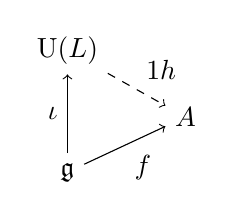
\begin{tikzpicture}
                \node (L) {$\lie$};
                \node[above =of L] (UL) {$\U(L)$};
                \node (A) at (1.5,0.7) {$A$};
                \draw[->] (L) --node[left] {$\iota$} (UL);
                \draw[->] (L) --node[below right] {$f$} (A);
                \draw[dashed,->] (UL) --node[above right] {$\Exists1 h$} (A);
            \end{tikzpicture}
        \]

        リー環$\lie$の包絡環を$(U(L), \iota)$とかく.
        \qed
    \end{definition}

    包絡環に関して次が成立します.
    \begin{Prop}
        包絡環は同型を除いてただ一つ存在する.
        \qed
    \end{Prop}
    
    次の手順で示します.
    \begin{Lem}
        包絡環に対して次が成り立つ.
        \begin{enumerate}
            \item 包絡環は存在すればただ一つ.
            \item $U \cong U(L)$ as ring $\Rightarrow$ $\exists \iota, (U, \iota)$をuniversalに出来る.
        \end{enumerate}
        \qed
    \end{Lem}
    
    \begin{Lem}
        $L$上のテンソル代数 $T(L) = \bigoplus_{n \geq 0}L^{\oplus n}$,
        $T$の両側イデアル $I := \langle X \otimes Y - Y \otimes X - [X, Y] \mid X, Y \in L \rangle$
        とする.
        この時,
        \begin{enumerate}
            \item $U(L) \cong T(L)/I$,
            \item $\iota: L \to U(L)$ は単射(ただし$\iota$は埋め込み).
        \end{enumerate}
        \qed
    \end{Lem}
    
    テンソル代数を両側イデアルで割って環を作るのは,生成元と基本関係式で環を定めるという構成方法です.きちんと述べると,
    \begin{Def}
        $X_1, \dots, X_n$を基底にもつ$\mathbb{C}$上のベクトル空間$V$. 
        そのテンソル環$T(V) = \bigoplus_{n \geq 0}V^{\oplus n} \ni R_1, \dots, R_m$.
        この時$R_1, \dots, R_m$で生成される両側イデアル: 
        \[
            I = \sum_{i = 1}^{m}T(V)R_iT(V)
        \]
        を考える (すなわち$I$は$R_1, \dots, R_m$を含む最小の両側イデアル).
        この時,
        \[
            T(V)/I
        \]
        を$X_1, \dots, X_n$を生成元とし,$R_1 = \cdots = R_m = 0$ を基本関係とする環という.
        \qed
    \end{Def}
    
    ここで包絡環の構成に戻れば,$U(L)$は$L$の基底$X_1, \dots, L_n$ を生成元とし,$X \oplus Y - Y \oplus X = [X, Y]$ を基本関係とする環とみなせます.特に$[X, Y] \in U(L)$に注意して,基本関係は$X_iX_j - X_jX_i = \sum C_{ij}^k X_k$と書き直せます.
    
    リー環の表現論は,包絡環の話にすることができます.
    \begin{Prop}
        $V_1, V_2$を$L$-加群,$f:V_1 \to V_2$を$L$-加群の準同型とする.この時,$f$は$U(L)$-加群の準同型でもある.
        \qed
    \end{Prop}
    
    \begin{Prop}
        $L$-Mod: リー環$L$の表現のなす圏,$U(L)$-Mod: 包絡環 $U(L)$の表現のなす圏とする.この時,関手$\mathcal{F}, \mathcal{G}$を次で定める.
        \begin{align*}
            \mathcal{F}: L\textrm{-mod} &\to U(L)\textrm{-mod}\\
            (\rho, V) &\to (\phi, V)\\
            f \in \Hom_L(V_1, V_2) &\to f \in \Hom_{U(L)}(V_1, V_2)
        \end{align*}
        \begin{align*}
            \mathcal{G}: U(L)\textrm{-mod} &\to L\textrm{-mod}\\
            (\phi, V) &\to (\phi, V)\\
            f \in \Hom_{U(L)}(V_1, V_2) &\to f \in \Hom_L(V_1, V_2)
        \end{align*}
        この時,$\mathcal{F}, \mathcal{G}$は圏の同型を与える.
        \qed
    \end{Prop}
    
    リー環はテンソル積表現を持つちます.
    \begin{Def}
        $L$の表現$(\rho_1, V_1), (\rho_2, V_2)$.
        $L$の表現とすると,$V_1 \bigoplus V_2$は
        \[
            \rho(X) = \rho_1(X) \oplus 1 + 1 \oplus \rho_2(X)
        \]
        で$L$の表現になる.これをテンソル積表現という.
        \qed
    \end{Def}
    
    リー環のテンソル積表現を包絡環の表現にすると,環のテンソル積になります.ここで,テンソル積表現を持つためには余積が与えられている必要があることを思い出しましょう..
    
    \begin{Prop}
        $\Delta: U(L) \to U(L) \otimes U(L)$ homで,
        \[
            \Delta \circ \iota(X) = \iota(X) \otimes 1 + 1 \otimes \iota(X)
        \]
        を満たすものがただ一つ存在して,$L$の任意のテンソル積表現$\rho = \rho_1 \oplus 1 + 1 \oplus \rho_2$に対応する$U(L)$の表現は$(\phi_1 \otimes \phi_2) \circ \Delta$.
        \[
            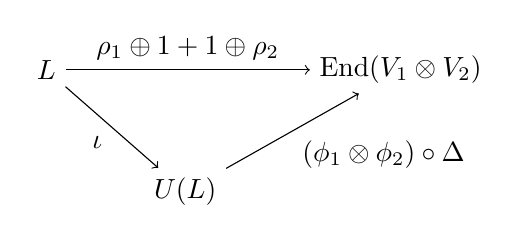
\begin{tikzpicture}[scale = 1.5]
                \node (L) {$L$};
                \node  at (3,0) (EL) {$\End(V_1 \otimes V_2)$};
                \node[below right  = of L] (U) {$U(L)$}; 
                
                \draw [->] (L) -- node[above] {$\rho_1 \oplus 1 + 1 \oplus \rho_2$}(EL);
                \draw [->] (L) -- node[below left] {$\iota$} (U);
                \draw [->] (U) -- node[below right] {$(\phi_1 \otimes \phi_2) \circ \Delta$} (EL);
            \end{tikzpicture}
        \]
        \qed
    \end{Prop}
    
    さて,この章のメインは次の定理です.
    \begin{Th}
        $(X_i)_{i \in I}$: $L$の基底.
        この時,
        \[
            \{X_{i1}\cdotsX_{im} \mid i1 \leq \cdots \leq im\}
        \]  
        は$U(L)$の基底を与える.
        \qed
    \end{Th}
  \end{document}
